%!TEX root = ../thesis.tex

\chapter{MHD Verification and Case-Specific Validation Results}
\label{chap:mhd-validation-results}

Chapter~\ref{chap:methodology} defines the reference hierarchy and the
diagnostics used here; each result below is conditional on its solver,
precision, device, grid and final time.

\section{Order verification against an exact solution}
\label{sec:ch4-cp-alfven}

The remaining cases admit no exact field, so they support self-refinement rates
but not an observed order of accuracy. The circularly polarised Alfv\'en wave
supplies one: it is an exact nonlinear solution at finite amplitude, since
$|\mathbf B|$ and the total pressure stay uniform. With $\rho=1$, $p=0.1$,
$B_x=1$, $\mathbf B_\perp=A(\sin2\pi x,\cos2\pi x)$ at $A=0.1$ and
$\mathbf v_\perp=-\mathbf B_\perp/\sqrt{\rho}$, the Alfv\'en speed is unity, so
the state at $t=1$ on the unit periodic domain is the initial condition
translated through one wavelength, that is, itself
\citep{toth_2000,gardinerStone2005ct}, and the final-minus-analytic difference
is true discretisation error. The data are $y$-independent and exactly
solenoidal by construction, with $\mathrm{divB}_{\max}$ below
$1.2\times10^{-13}$ on every grid, so GLM cleaning does not enter.

Refining from $N=32$ to $N=512$, the transverse field mean $L_1$ error falls
from $6.565\times10^{-3}$ to $4.288\times10^{-5}$, a fitted order of $1.818$
with $R^2=0.9997$ (Figure~\ref{fig:ch4-cp-alfven}). The pairwise orders rise
monotonically, $1.706$, $1.822$, $1.844$, $1.886$, approaching second order
from below as the limiter's influence near the extrema of a smooth wave
recedes. The fp64 and fp32 groups agree to four significant figures and the CPU
and GPU groups are identical, so the CUDA HLL path is order-verified rather
than merely compared against the host. This is the only accuracy statement here
resting on an exact field, and it does not transfer to the cases below.

\begin{figure}[htbp]
\centering
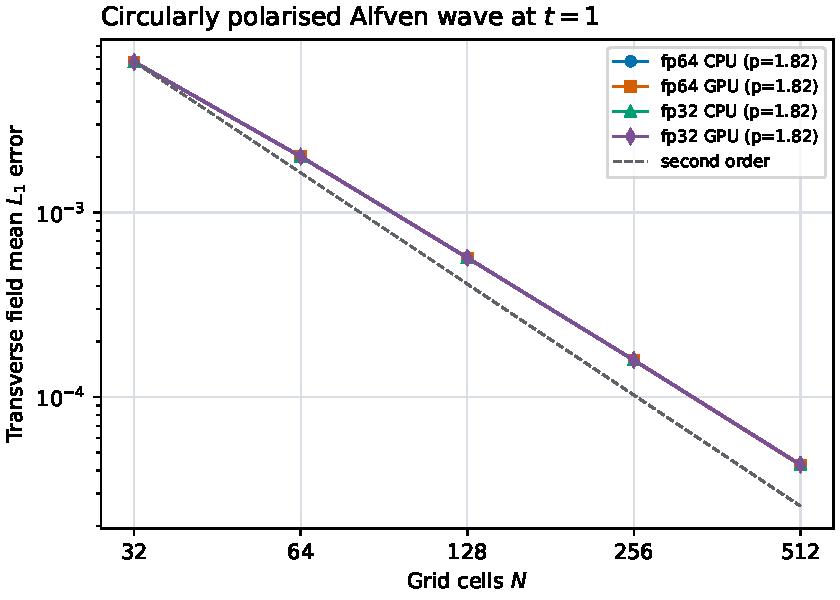
\includegraphics[width=0.68\textwidth]{Figs/report2/ch4_cp_alfven_convergence}
\caption[Circularly polarised Alfv\'en wave convergence]{\textbf{Circularly
polarised Alfv\'en wave convergence.} Transverse field mean $L_1$ error against
the exact solution at $t=1$, HLL, for both precisions on both devices; the four
series overlap. The dashed line marks second order.}
\label{fig:ch4-cp-alfven}
\end{figure}

\section{Brio--Wu numerical-reference assessment}
\label{sec:ch4-brio-wu}

Three fp64 grids of the coplanar MHD Riemann problem of \citet{brio_wu_1988}
were compared against an $N=8000$ numerical comparator, conservatively
downsampled by averaging the $8000/N$ fine cells in each candidate cell. From
$N=200$ to $N=800$ the density mean $L_1$ difference fell from
$1.481\times10^{-2}$ to $5.642\times10^{-3}$ and $L_2$ from
$3.642\times10^{-2}$ to $1.923\times10^{-2}$, with
$\mathrm{divB}_{\max}\leq4.441\times10^{-14}$ throughout; least-squares fits of
$\log_2 E=a-q\log_2 N$ give $q=0.70$ in $L_1$ and $0.46$ in $L_2$. Since the
order is verified separately (Section~\ref{sec:ch4-cp-alfven}), these rates
measure what discontinuities cost it. The standard smearing estimate for a
linearly degenerate contact, at which an order-$p$ monotone scheme converges in
$L_1$ as $h^{p/(p+1)}$ \citep{toro2009,leveque_2002}, gives $h^{2/3}$ for
$p=2$, close to the observed $0.70$; the compound wave and the comparator's
shared discretisation bias also admit pseudo-convergence
\citep{torrilhon2003pseudo}.

The $N=800$ profiles in Figure~\ref{fig:ch4-brio-profiles} reproduce the
sequence of \citet{brio_wu_1988} --- fast rarefaction, slow compound wave,
contact, slow shock, fast rarefaction --- with the contact and slow shock
visibly displaced and smeared against the comparator, where the mean $L_1$
difference concentrates.

\begin{figure}[htbp]
\centering
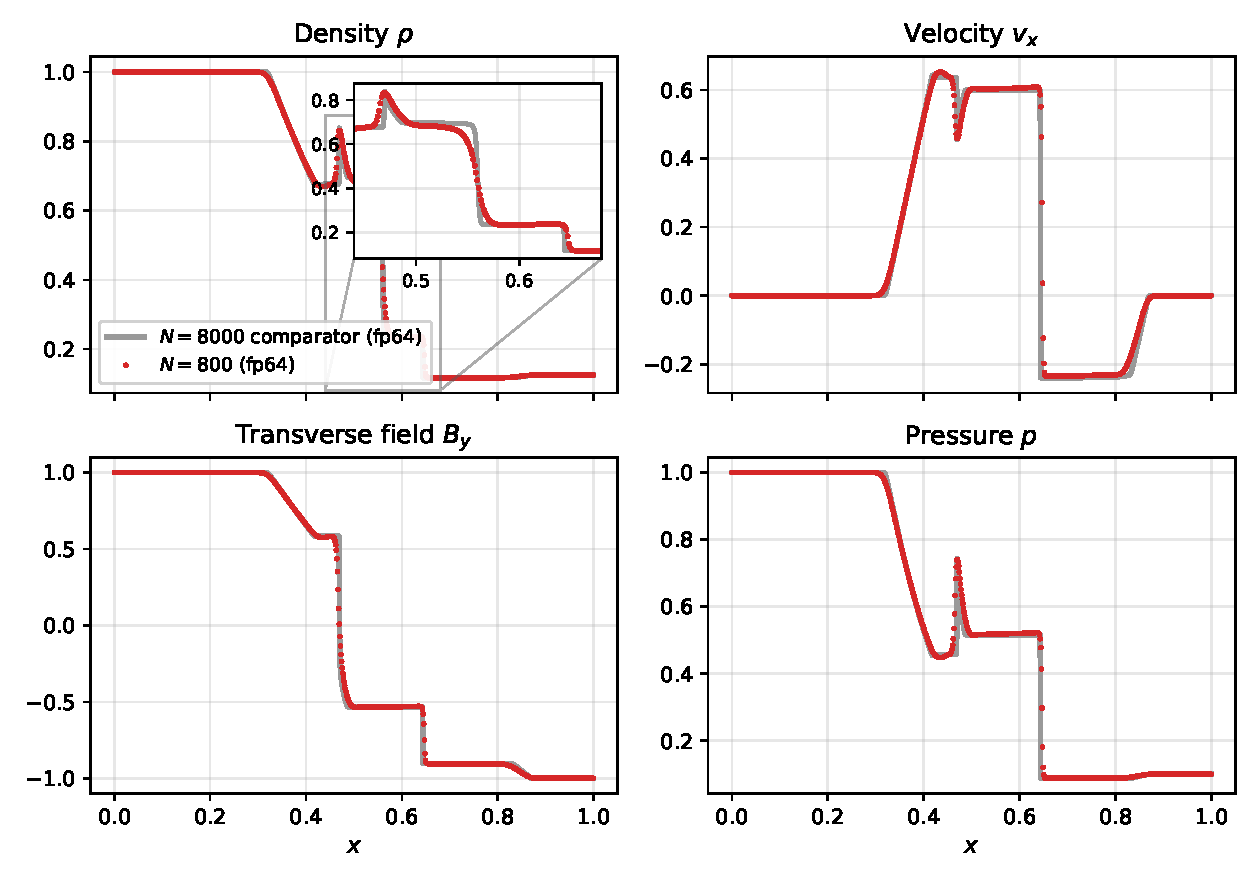
\includegraphics[width=\textwidth]{Figs/report2/ch4_brio_wu_profiles}
\caption[Brio--Wu final-state profiles]{\textbf{Brio--Wu final-state profiles.}
HLL fp64 density, normal velocity, transverse magnetic field and pressure at
$t=0.1$: $N=800$ candidate and same-HLL $N=8000$ numerical comparator.}
\label{fig:ch4-brio-profiles}
\end{figure}

\section{Two-dimensional property verification and divergence control}
\label{sec:ch4-invariance-glm}

An $800\times4$ embedding of Brio--Wu preserved a transversely constant state
exactly, every row identical component by component. Against the
one-dimensional run the mean and maximum absolute density differences were
$3.550\times10^{-4}$ and $7.034\times10^{-3}$, below the predeclared $10^{-3}$
and $10^{-2}$ and explained by the $y$-direction fast speed requiring 861
rather than 759 steps.

Cleaning was tested directly on a state that is non-solenoidal by construction:
a Gaussian normal-field bump $B_x=B_0\exp(-r^2/\sigma^2)$ at $(0.5,0.5)$ on a
doubly-periodic $128^2$ square, for which divergence is of order unity. At
$t=0.5$, $\max|\nabla\!\cdot\!\mathbf{B}|$ was 3.030 undamped, 0.2678 at
$c_r=0.18$ and 0.8429 at $c_r=0.36$ (Figure~\ref{fig:ch4-glm-divergence});
since the damping rate is $c_h/c_r$, the chosen $c_r=0.18$ damps the more
strongly, consistent with its smaller terminal maximum.

% Source PDF SHA-256:
% ca1c0d20572818a015eb394aa3bb43786b874ce4604e889fb310f5ec4e15c442
\begin{figure}[htbp]
\centering
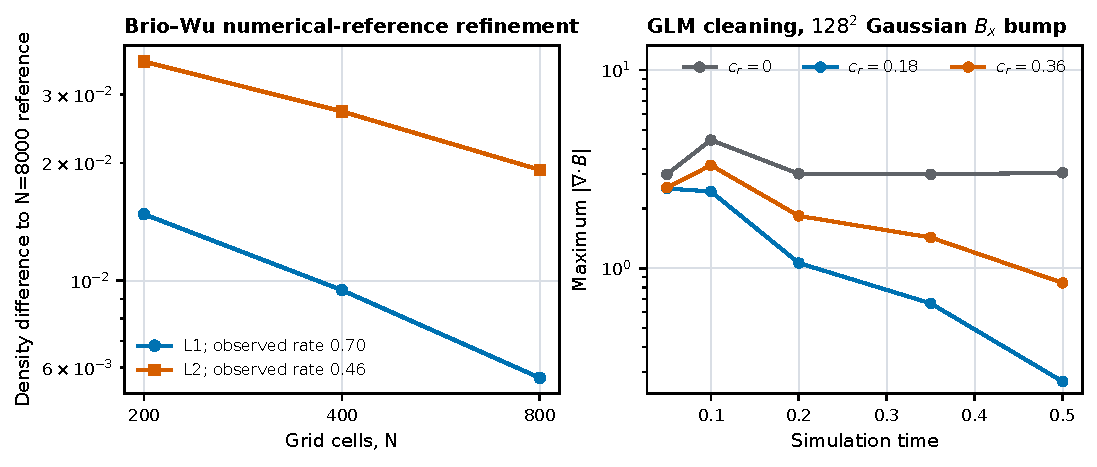
\includegraphics[width=0.82\textwidth,viewport=266.072 0 532.144 200,clip]{Figs/report2/ch4_validation_refinement_glm}
\caption[GLM divergence diagnostic]{\textbf{GLM divergence diagnostic.}
Maximum divergence for the doubly-periodic $128^2$ Gaussian normal-field bump
(HLL, fp64, CFL 0.4), one run per stopping time; $c_r=0$ is the undamped
control.}
\label{fig:ch4-glm-divergence}
\end{figure}

\section{Matched CPU/GPU implementation verification}
\label{sec:ch4-cpu-gpu-validation}

Case, grid, precision, arithmetic and update order were matched across separate
CPU and CUDA HLL implementations. Table~\ref{tab:ch4-cpu-gpu} reports four
pairs, Brio--Wu at $800\times1$ and Orszag--Tang at $256^2$ in fp32 and fp64,
each repeated five times, all giving zero maximum ULP and zero absolute
$L_\infty$ difference. The $c_h$ reduction was reordered into a parallel GPU
maximum tree, which cannot accumulate rounding, and device contraction was
disabled to match the host (Section~\ref{sec:ch2-execution}), so the agreement
holds for that build recipe. A shared defect would still agree bit for bit.

% Generated by scripts/figures/report2_chapter4_cpu_gpu_table.py
% Source: experiments/week16/cpu_gpu_hardware_axis/summary.json
\begin{table}[htbp]
\centering
\small
\begin{tabularx}{\textwidth}{@{}llccccX@{}}
\toprule
Case & Precision & Grid & CPU/GPU steps & $\mathrm{ULP}_{\max}$ & $L_\infty$ & Verified output \\
\midrule \addlinespace[2pt]
Brio--Wu & fp64 & $800\times1$ & 759/759 & 0 & 0 & HLL saved state \\
Brio--Wu & fp32 & $800\times1$ & 759/759 & 0 & 0 & HLL saved state \\
Orszag--Tang & fp64 & $256^2$ & 806/806 & 0 & 0 & HLL saved state \\
Orszag--Tang & fp32 & $256^2$ & 806/806 & 0 & 0 & HLL saved state \\
\bottomrule
\end{tabularx}
\caption[Matched CPU/GPU MHD implementation verification]{\textbf{Matched CPU/GPU MHD implementation verification.} Same-precision CPU and GPU HLL runs used the same case configuration on the recorded workstation. Steps are reported as CPU/GPU, and $L_\infty$ denotes the absolute difference between saved states. All four comparisons are bit-identical.}
\label{tab:ch4-cpu-gpu}
\end{table}


\section{Orszag--Tang validation}
\label{sec:ch4-orszag-tang}

The Orszag--Tang test uses the periodic unit-square rescaling of
\citet{toth_2000}, and the HLL runs at $128^2$, $256^2$, and $512^2$ completed
with finite, positive states. The divergence diagnostic is dimensional, so the
ladder is read in grid units: scaled by cell width the domain mean falls about
fivefold, so cleaning works wherever the field is smooth, while the maximum
barely moves, staying near $1.4\%$ of $B_0$ per cell width. Without
explicit resistivity ideal MHD current sheets keep thinning under refinement,
leaving a sheet a few cells across whose central-difference residual scales as
$1/h$, so the peak stays pinned at the grid scale and its raw growth reflects
the diagnostic's dimensions rather than lost divergence control. The fp64 HLL
$256^2$--$512^2$ pair retained zero relative mass drift, a necessary but weak
check, and its temperature field preserved the interacting-shock and
current-sheet topology of published calculations
\citep{toth_2000,bard_dorelli_2014} (Figure~\ref{fig:ch4-ot-morphology}).

\begin{figure}[htbp]
\centering
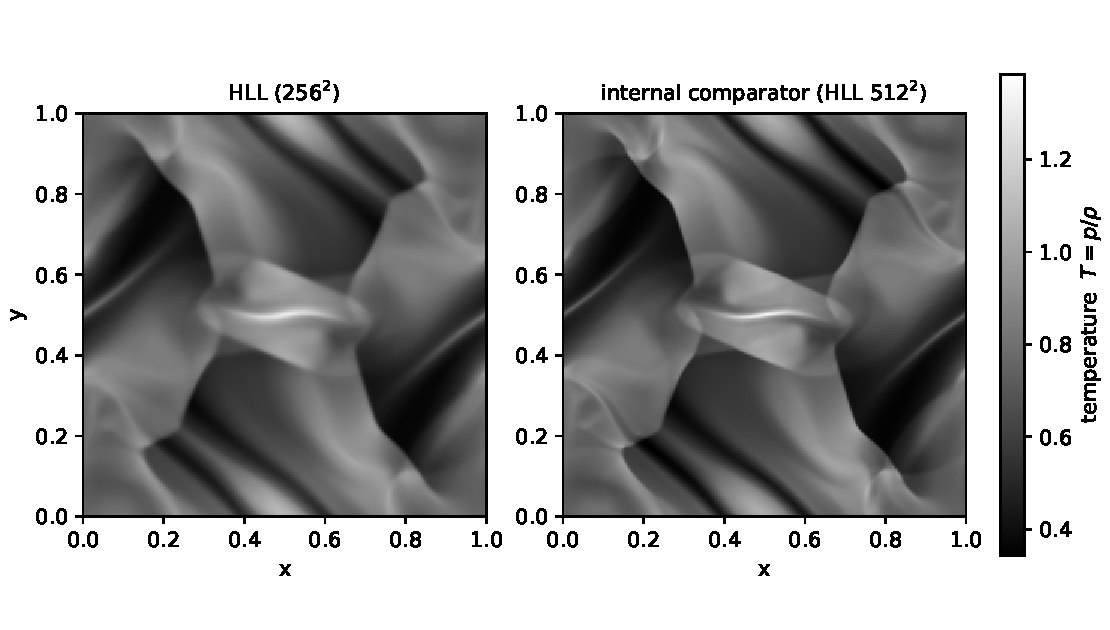
\includegraphics[width=\textwidth]{Figs/report2/ch4_orszag_tang_morphology}
\caption[Orszag--Tang temperature morphology]{\textbf{Orszag--Tang temperature
morphology.} HLL fp64 temperature at $256^2$ and the internal higher-resolution
$512^2$ HLL comparator at $t=0.5$, plotted on one scale. Over $128^2$, $256^2$
and $512^2$ the cell-width-scaled divergence mean falls $1.07\times10^{-3}$,
$4.79\times10^{-4}$, $2.02\times10^{-4}$, while its maximum moves only from
0.0136 to 0.0145 to 0.0151.}
\label{fig:ch4-ot-morphology}
\end{figure}

Figure~\ref{fig:ch4-resolution-precision} gives the adjacent-grid diagnostic
$p=\log_2(E_{\mathrm{coarse}}/E_{\mathrm{fine}})$, with $E$ the density
mean-$L_1$ difference between successive grids, so $p=1$ if that difference
halves on each doubling and $p=2$ if it quarters. The two-dimensional update
composes its sweeps as a fixed $x$-then-$y$ Lie splitting, which is first order
as a multidimensional split (Section~\ref{sec:ch2-mhd-glm}), so the reference
here is $p\simeq1$ rather than 2, and minmod limiting lowers it further
wherever it activates. For fp64 HLL the differences were 0.1203 and 0.07722,
giving $p\simeq0.639$, and for HLLD \citep{miyoshi_kusano_2005} 0.07515 and
0.04182, giving $p\simeq0.846$; the fp32 values agreed at the displayed
precision. Both fall below the reference, as shocks and current sheets keeping
the limiter active would produce, and for HLL the globally clamped wave speed
of Section~\ref{sec:ch2-riemann} adds Rusanov dissipation everywhere on top of
that.

Because the two ladders ran at different time steps, HLL was re-run at the HLLD
setting. At CFL 0.2 it gives $p\simeq0.640$ for Orszag--Tang and $0.917$ for
Kelvin--Helmholtz, against $0.639$ and $0.919$ at CFL 0.4, so the rates are
insensitive to the time step across this range and the CFL asymmetry was not
the confound it appeared to be. At a matched step HLLD attains the higher rate
on both cases, $0.846$ against $0.640$ and $1.442$ against $0.917$, so the
ordering is a solver comparison after all, consistent with the clamped HLL flux
carrying extra dissipation everywhere.

An exploratory fp64 HLLD run at $512^2$ terminated with diagnosed negative
pressure at CFL 0.4 and again at 0.2, so reducing the time step was not the
fix. Pressure is recovered as
$p=(\gamma-1)[E-\rho|\mathbf{v}|^2/2-|\mathbf{B}|^2/2]$, so where magnetic and
kinetic energy dominate $E$ the subtraction cancels leading digits and the
relative error in $p$ is amplified by roughly $E/p$ \citep{higham_2002}. The
guard detects a cancellation-sensitive recovery, though whether its threshold
depends on the working precision was not tested. With the per-line first-order
HLL fallback enabled the ladder completed at all three grids, and
instrumentation shows how little of it that fallback carries: the recomputation
fired twice in $3\,355\,648$ line updates at $512^2$ and not at all at $256^2$
or on Brio--Wu, while HLLD's fourteen degeneracy guards never fired in
$1.7\times10^{9}$ interface evaluations. The $512^2$ diagnostics therefore
describe HLLD almost everywhere, the fallback acting as a point repair rather
than a regime. Figure~\ref{fig:ch4-ot-solver-comparison} shows where the two
$256^2$ fields differ against the same HLL $512^2$ context.

\begin{figure}[htbp]
\centering
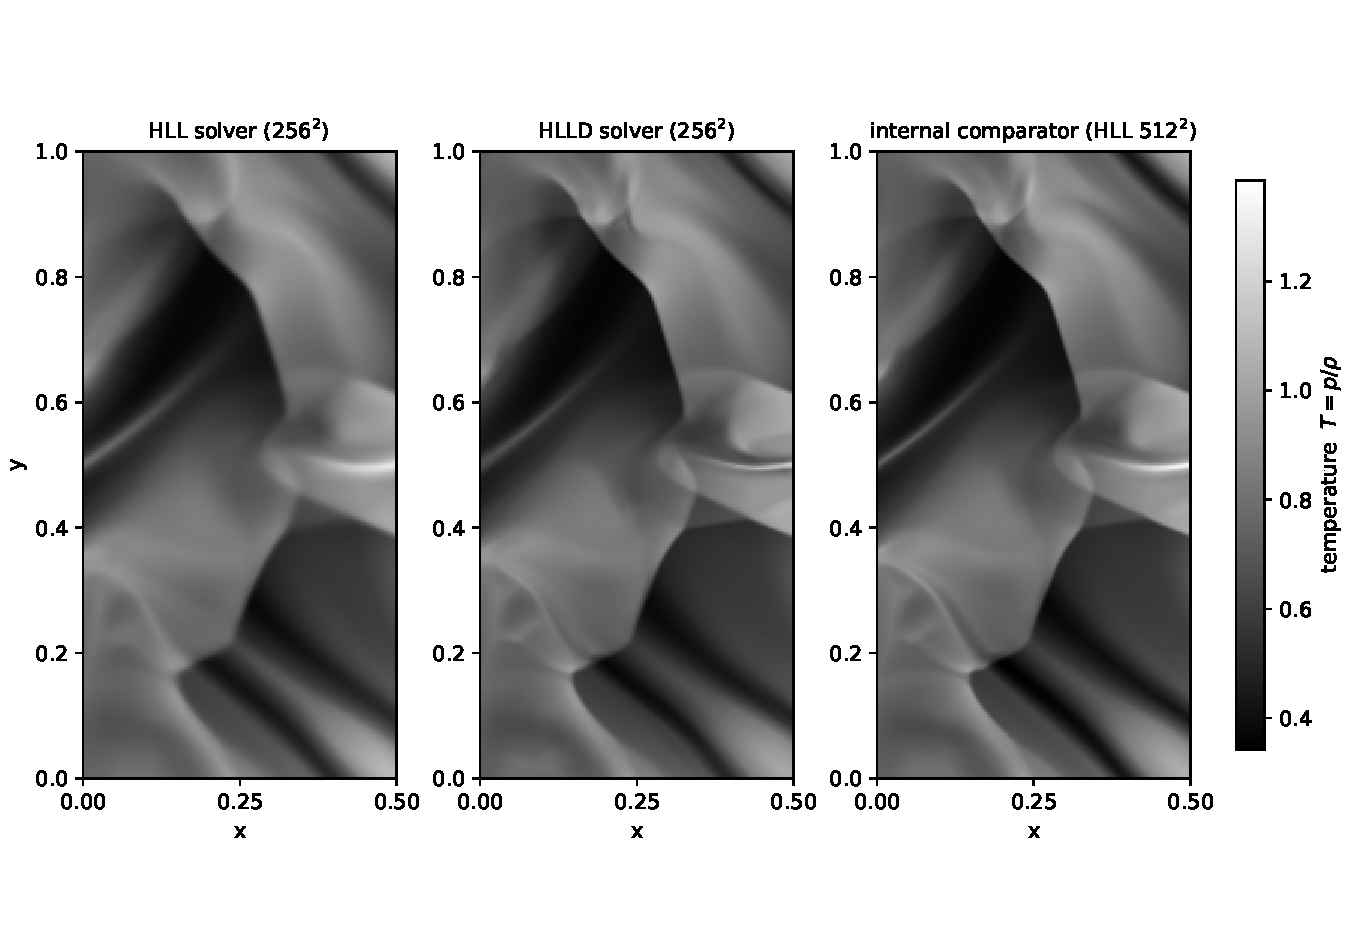
\includegraphics[width=\textwidth]{Figs/report2/ch4_orszag_tang_solver_comparison}
\caption[Orszag--Tang HLL/HLLD field comparison]{\textbf{Orszag--Tang
HLL/HLLD field comparison.} Left-half temperature at $t=0.5$ for fp64 HLL and
HLLD at $256^2$, with the internal HLL $512^2$ field as refinement context.}
\label{fig:ch4-ot-solver-comparison}
\end{figure}

% Source PDF SHA-256:
% 36c516bdd93a30a13861430752bd7b7f732f1f12b91253ae616fc59b8850c017
\begin{figure}[htbp]
\centering
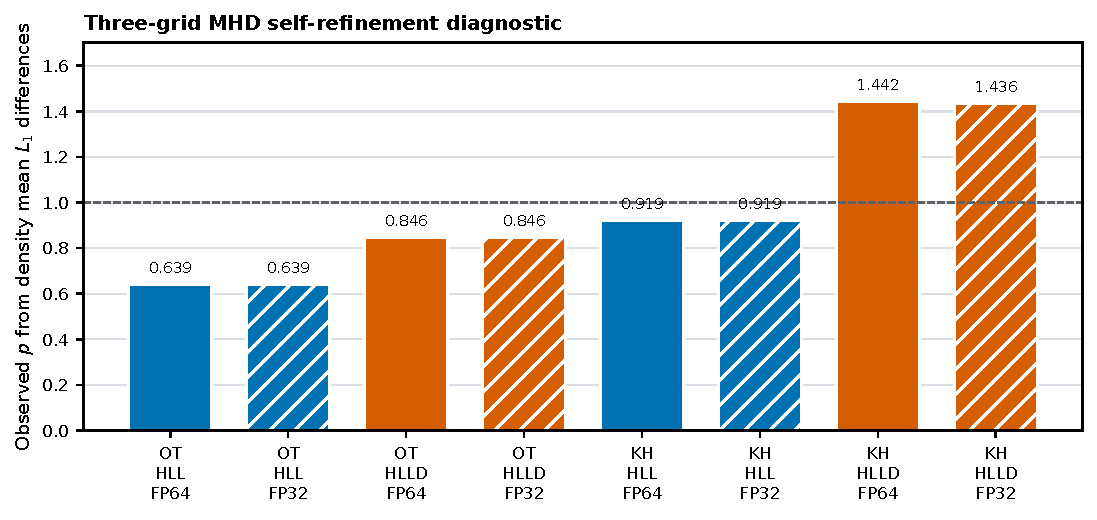
\includegraphics[width=\textwidth]{Figs/report2/ch4_resolution_precision}
\caption[Three-grid MHD resolution diagnostics]{\textbf{Three-grid MHD
resolution diagnostics.} Adjacent grids are conservatively block-averaged
before the density mean $L_1$ difference is formed. HLL uses CFL 0.4 and HLLD
uses CFL 0.2; the matched-CFL comparison is given in the text. The dashed line
marks $p=1$, the first-order behaviour expected from the fixed directional
splitting: bars near it are splitting-limited, bars below it lose further order
where limiting is active, and the two Kelvin--Helmholtz HLLD bars above it
indicate that three grids have not reached an asymptotic regime rather than
better-than-first-order accuracy.}
\label{fig:ch4-resolution-precision}
\end{figure}

\section{Kelvin--Helmholtz validation}
\label{sec:ch4-kelvin-helmholtz}

The initial data (Equation~\ref{eq:ch3-ic-kh}) are a smooth double shear layer
of width $a=0.025$, a single-wavelength $\sin(2\pi x)$ seed and a uniform
flow-aligned field at Alfv\'en Mach number 5. In the regime of
\citet{frankEtAl1996kh} such a weak aligned field cannot suppress the
instability, though it can modify the nonlinear stage; at a sonic Mach number
near 0.39 the case is subsonic, so density is a low-contrast diagnostic here. A
separate reproduction tested the linear stage directly. On the smooth
unstratified initial condition of \citet{lecoanetEtAl2016kh}, with
$\mathbf{B}=0$ so the solver reduces to inviscid hydrodynamics, the $k=2\pi$
mode amplitude of \citet{tricco2019kh} grew at 2.193 over $t\in[0.25,1.0]$ at
$128\times256$ with $R^2=0.990$, against the published linear value of 3.227
\citep{berlokPfrommer2019kh}. Growth is recovered with the right sign but is
32\% slow, the expected direction for the globally clamped, Rusanov-like HLL
path on a marginally resolved layer. That check bounds linear hydrodynamic
behaviour only, using a different initial condition and no field.

All solver--precision groups completed at $128^2$, $256^2$, and $512^2$ with
finite, positive states. Scaled by cell width and by $B_0=0.1$, both divergence
maxima fall monotonically, from $4.7\times10^{-5}$ to $1.8\times10^{-5}$ for
HLL and from $7.1\times10^{-4}$ to $1.0\times10^{-4}$ for HLLD: two to three
orders tighter than Orszag--Tang's $1.4\%$, and tightening under refinement
rather than pinned at the grid scale, because the shear layer keeps a fixed
width that refinement resolves. HLLD's maximum stays about an order of
magnitude above HLL's, comparing a uniformly smoothed field with a sharper one,
so low dissipation and tight discrete divergence control are not obtained
together.

For fp64 HLL and HLLD, the adjacent-grid density differences shrink with
$p=0.919$ and $p=1.442$. On this smooth field the HLL value sits close to the
splitting-limited reference of Section~\ref{sec:ch4-orszag-tang}, whereas the
HLLD value exceeding one indicates that three grids have not reached an
asymptotic regime rather than a better-than-first-order method. These remain
self-refinement rates, not solution error; only
Section~\ref{sec:ch4-cp-alfven} measures the latter.
